\documentclass{article}
\usepackage{amsmath}
\usepackage{amssymb}
\usepackage{graphicx}
\usepackage{hyperref}
\usepackage[version=4]{mhchem}


\begin{document}
In triangle \(A B C, B M\) is the median on \(A C\). \(A E\) and \(A F\) trisect \(B C\) and meet \(B M\) at \(G\) and \(H\), respectively. \(B G: G H: H M=x: y: z\). Find the value of \(x\) \(+y+z\), where \(x, y\), and \(z\) are positive integers relatively prime.

Solution: 10 .\\
Method 1:\\
Connect \(F M\). We see that \(F M / / A E\) since \(M\) is the midpoint of \(A C\) and \(F\) is the midpoint of \(E C\).\\
\centering
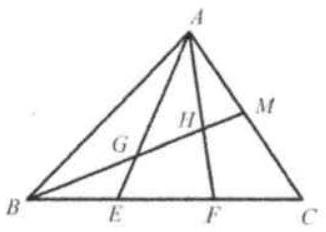
\includegraphics[width=\textwidth]{images/118.jpg}\\
\(M F=\frac{1}{2} A E=\frac{1}{2}(G E+A G)=2 G E\). So \(A G=3 G E\) and \(M F=\frac{2}{3} A G\).\\
We know that \(A G / / M F\). So \(\triangle A G H \sim \triangle F M H\). \(\frac{A G}{M F}=\frac{G H}{H M}=\frac{3}{2}\).\\
We also know that \(B G=G M\). So \(B G: G H: H M=5: 3: 2\). The answer is \(5+3+\) \(2=10\).


\begin{center}
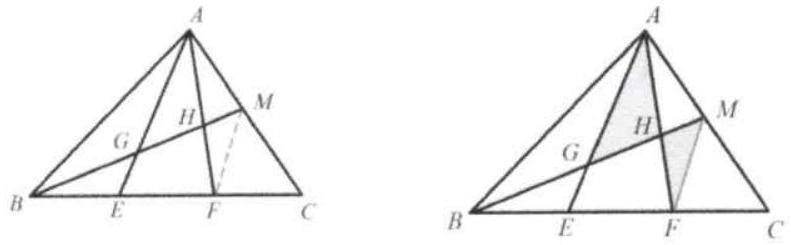
\includegraphics[width=\textwidth]{images/119.jpg}
\end{center}

Method 2:\\
Draw \(C P / / A F\) and \(C Q / / A E\) through point \(C\) and to meet the extension of \(B M\) at \(P\) and \(Q\), respectively. We see that \(\triangle A G M \equiv \triangle C Q M\)\\
\((\angle G A M=\angle Q C M, A M=M C, \angle A M G=\angle C M Q)\).\\
So \(G M=M Q\). Similarly, we get \(H M=M P\).\\
Let \(B G=x, G H=y, H M=z\).\\
\centering
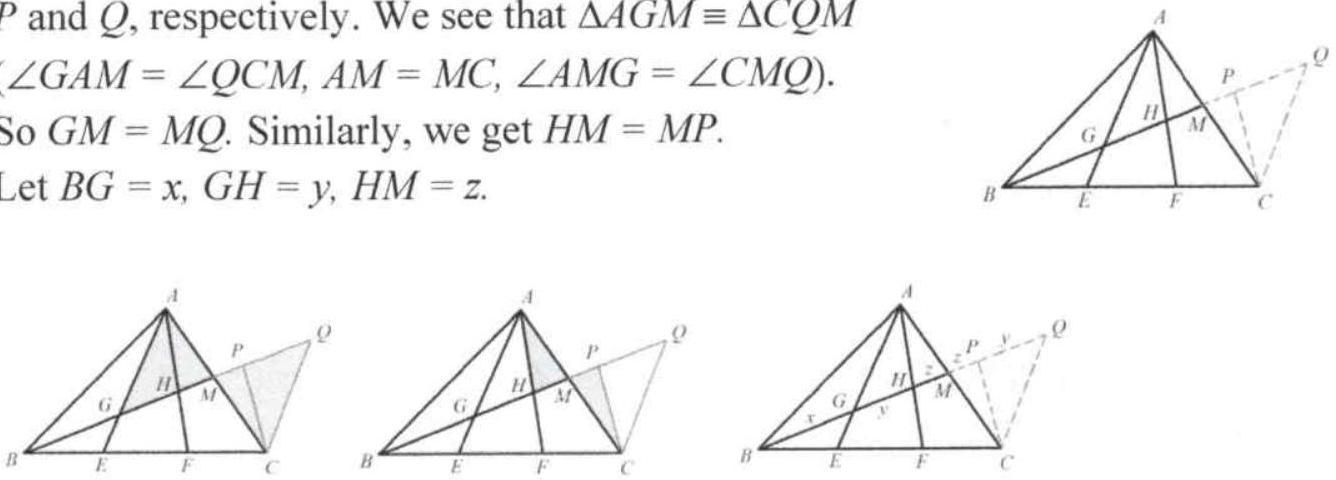
\includegraphics[width=\textwidth]{images/119(2).jpg}

We know that \(G E / / C Q\). So \(\triangle B E G \sim \triangle B C Q . \frac{B G}{B Q}=\frac{B E}{B C}=\frac{1}{3}\).\\
Therefore \(x=y+z\)\\
\centering
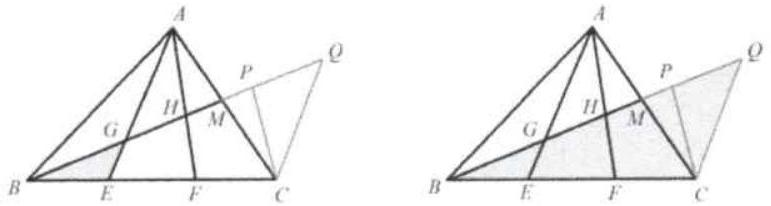
\includegraphics[width=\textwidth]{images/119(1).jpg}

We know that \(H F / / P C\). So \(\triangle B F H \sim \triangle B C P\). \(\frac{B H}{B P}=\frac{B F}{B C}=\frac{2}{3}\)\\
\(\Rightarrow \frac{x+y}{2 x+z}=\frac{2}{3}\).\\
Therefore \(3 y=2 z+x\)


Substituting (1) into (2): \(\frac{y}{z}=\frac{2}{3}\). So \(x: y: z=5: 3: 2\). The answer is \(5+3+2=\) 10.\\
\centering
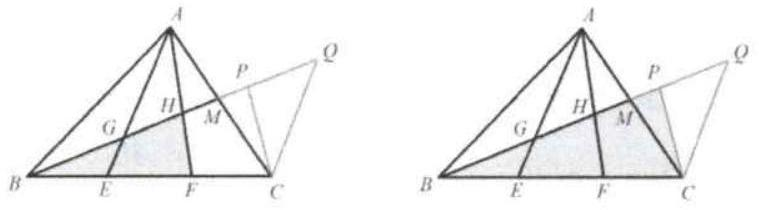
\includegraphics[width=\textwidth]{images/120(2).jpg}

Method 3:\\
Extend \(B M\) to \(N\) such that \(M N=B M\). Connect \(A N, C N . A B C N\) is a parallelogram because the diagonals bisect each other. Thus \(A F / / B C . A N=B C=3 B E\).

We know that \(A N / / B C\). So \(\triangle B E G \sim \triangle N A G\).\\
\(\frac{N G}{B G}=\frac{A N}{B E}=3\). So \(N G=3 B G\).\\
\centering
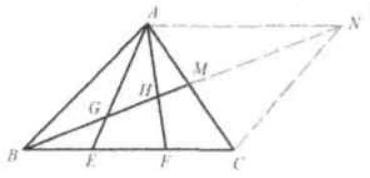
\includegraphics[width=\textwidth]{images/120(1).jpg}\\
\(B N=B G+G N=4 B G\).\\
\(B G=B N / 4\).\\
We know that \(A N / / B C\). So \(\triangle A N H \sim \triangle F B H\). \(\frac{N H}{B H}=\frac{A N}{B F}=\frac{3}{2}\). So \(N H=3 B H / 2\).\\
\(B N=B H+H N=5 B H / 2\).\\
So \(B H=2 B N / 5\).\\
Thus \(G H=B H-B G=\frac{2}{5} B N-\frac{1}{4} B N=\frac{3}{20} B N\).\\
\(H M=B M-B H=\frac{1}{2} B N-\frac{2}{5} B N=\frac{1}{10} B N\).\\
\(B G: G H: H M=\frac{1}{4}: \frac{3}{20}: \frac{1}{10}=5: 3: 2\)\\
The answer is \(5+3+2=10\).\\
\centering
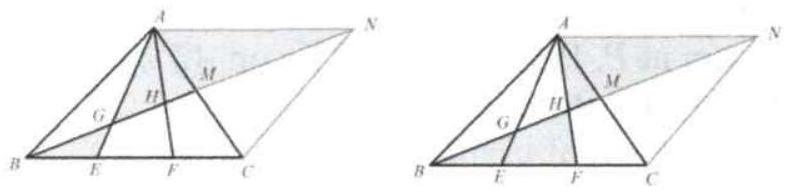
\includegraphics[width=\textwidth]{images/120.jpg}



\end{document}
